\documentclass[12pt]{article}
\usepackage{amsmath}
\usepackage{graphicx}

%\setlength\parindent{20pt} %% Do not touch this

\title{Homework 1} 

\author{Geneva Porter\\ 
MATH-693B Numerical Partial DIfferential Equations\\}

\date{February 10, 2020} 
\begin{document}
\maketitle

\section*{1.1.1}

Consider the initial value problem for the equation
$$
u_{t}+a u_{x}=f(t, x)
$$
$$
\text { with } u(0, x)=0 \text { and } \quad f(t, x)=\left\{\begin{array}{ll}
{1} & {\text { if } x \geq 0} \\
{0} & {\text { otherwise }}
\end{array}\right.
$$
Assume that $a$ is positive. Show that the solution is given by
$$
u(t, x)=\left\{\begin{array}{ll}
{0} & {\text { if } x \leq 0} \\
{x / a} & {\text { if } x \geq 0 \text { and } x-a t \leq 0} \\
{t} & {\text { if } x \geq 0 \text { and } x-a t \geq 0}
\end{array}\right.
$$

\subsubsection*{Solution}

When $f(t,x)=0$, we have the unique solution $u(t,x) = u_0(x-at)$. This gives the answer $u_0(x-at) = u(0, x-at) = 0$, which is the indicated solution for all $x<0$. 

For $f(t,x)=1$ and $x-at <0$, we can show that the solution $u(t,x)=x/a$ is valid. Observe:


\begin{equation*}
\begin{aligned}
u(t,x) = \frac{x}{a} ~~~ \longrightarrow ~~~ u_t = 0 ~~~ \text{and} ~~~ u_x = \frac{1}{a}
\end{aligned}
\end{equation*}

\noindent Plugging this into our problem, we see that the result is $0 +a(1/a) = 1$, which is true. So this solution is correct.

For $f(t,x)=1$ and $x-at \geq 0$, let's change variables so that

$$ \tau=t ~~~~~\text{and} ~~~~~ \xi=x-at ~~~ \longrightarrow ~~~ x = \xi +a\tau.$$

\noindent Now we have $\tilde{u}(\tau, \xi) = u(t,x)$, and it follows that

\begin{equation*}
\begin{aligned}
	 \frac{\partial\tilde{u}}{\partial\tau} &= \frac{\partial t}{\partial\tau}u_t + \frac{\partial x}{\partial\tau}u_x\\
	 &= u_t + au_x = f(\tau, \xi+a\tau).
\end{aligned}
\end{equation*}

\noindent With $\frac{\partial\tilde{u}}{\partial\tau}=f(\tau, \xi+a\tau)$, we can solve this as an ordinary differential equation, which has the following solution:

\begin{equation*}
\begin{aligned}
	\tilde{u}(\tau,\xi)& = u_0(\xi) + \int_0^\tau f(\sigma, \xi+a\sigma) d\sigma ~~~ \longrightarrow \\
	u(t,x) &= u_0(x-at) + \int_0^t f(s,x-a(t-s)) ds\\
	&= 0 + \int_0^t ds = \left.\frac{}{}s\right|_0^t = t
\end{aligned}
\end{equation*}

And we see that this is indeed the solution we were seeking.




\section*{1.3.1}

For values of $x$ in the interval $[-1,3]$ and $t$ in $[0,2.4],$ solve the one-way wave equation $u_{t}+u_{x}=0$ with the initial data
$$u(0, x)=\left\{\begin{array}{ll}
{\cos ^{2} \pi x} & {\text { if }|x| \leq \frac{1}{2}} \\
{0} & {\text { otherwise }}
\end{array}\right.$$
and the boundary data $u(t,-1)=0.$
Use the following four schemes for $h=1 / 10,~1 / 20,$ and $1 / 40$:
\begin{enumerate}
	\item
	\begin{enumerate}
		\item Forward-time backward-space scheme $(1.3 .2)$ with $\lambda=0.8$
		\item Forward-time central-space scheme $(1.3 .3)$ with $\lambda=0.8$
		\item Lax-Friedrichs scheme $(1.3 .5)$ with $\lambda=0.8$ and 1.6
		\item Leapfrog scheme $(1.3 .4)$ with $\lambda=0.8$.
	\end{enumerate}
\end{enumerate}





\subsubsection*{(a) Forward Time, Backward Space}
\vspace{-1mm}
Figure (1) shows this scheme. Notice that the approximate solution has a significant error at first, but is still "useful" (see video, emailed). For $h=1/10$, the largest error is 0.3094. For $h=1/20$, the error is 0.1888. For $h=1/40$, the error is 0.1055. As the density of the mesh doubles, the error reduces by roughly half.

\begin{figure}
	\centering
	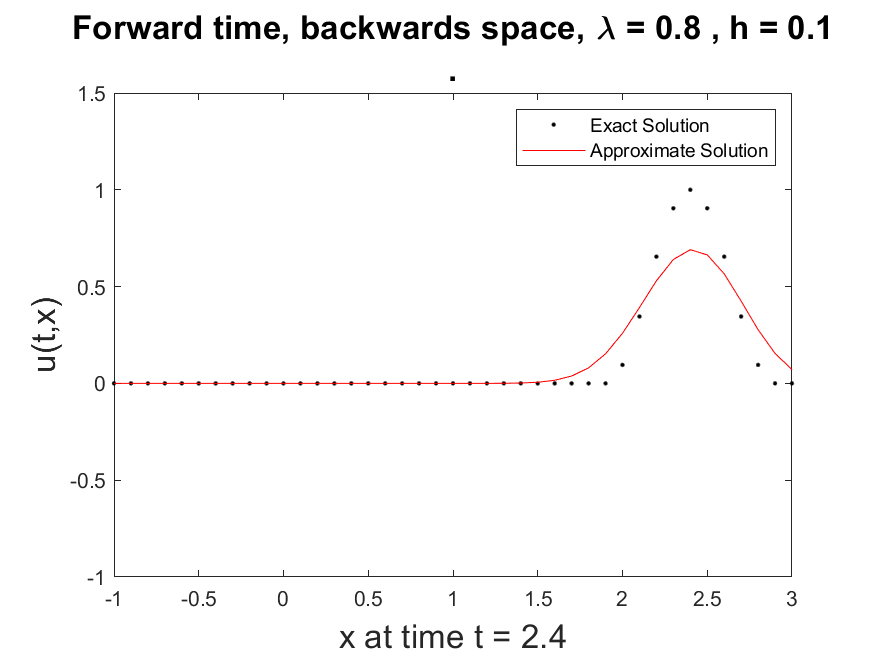
\includegraphics[width=.6\linewidth]{./code/a_forward_time_backward_space_1_10th.png}	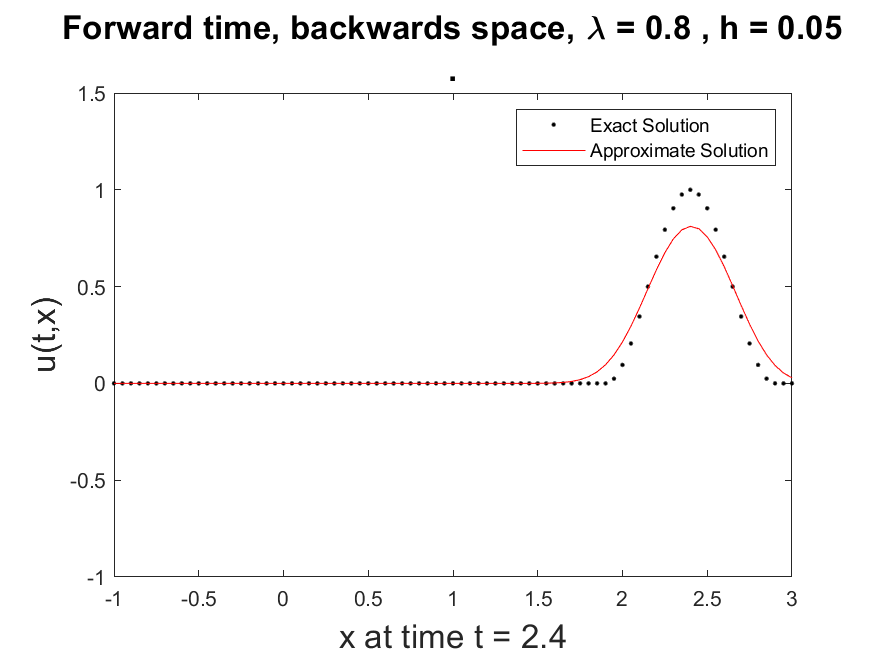
\includegraphics[width=.6\linewidth]{./code/a_forward_time_backward_space_1_20th.png}
	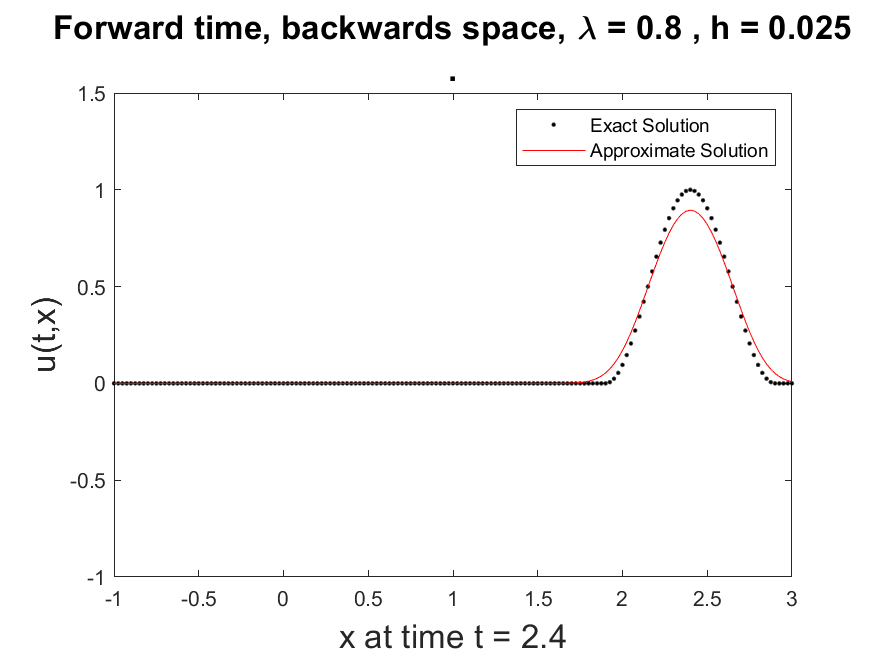
\includegraphics[width=.6\linewidth]{./code/a_forward_time_backward_space_1_40th.png}
	\caption{Forward time, backward space scheme at $t=2.4$ for $h-1/10, h=1/20$, and $h=1/40$, respectively}
\end{figure}

\subsubsection*{(b) Forward Time, Central Space}
\vspace{-1mm}
Figure (2) shows this scheme. Notice that the approximate solution explodes to infinity  (see video in code). For $h=1/10$, the solution exceeds a value of 5 after about 1.76 seconds. For $h=1/20$, the solution exceeds 5 after about 1.2 seconds. For $h=1/40$, the solution passes 5 after about .72 seconds. As the density of the mesh doubles, the solution becomes useless more quickly.

\begin{figure}
	\centering
	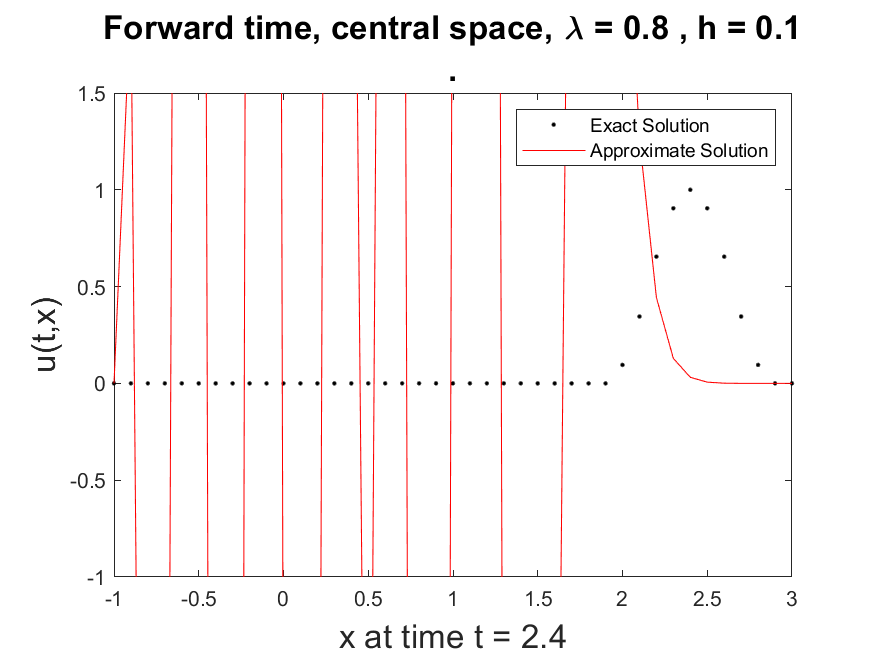
\includegraphics[width=.6\linewidth]{./code/b_forward_time_central_space_1_10th.png}	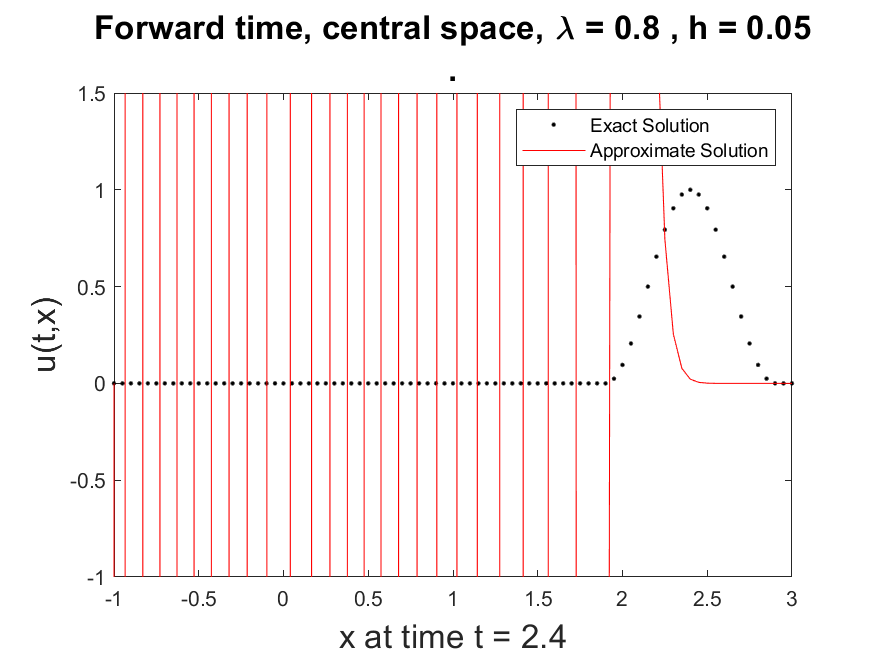
\includegraphics[width=.6\linewidth]{./code/b_forward_time_central_space_1_20th.png}
	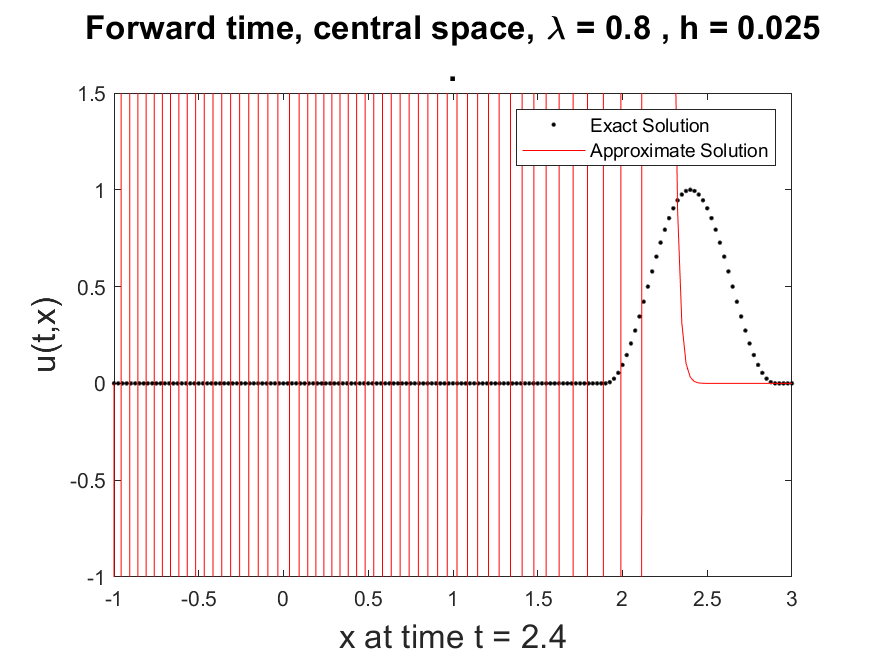
\includegraphics[width=.6\linewidth]{./code/b_forward_time_central_space_1_40th.png}
	\caption{Forward time, central space scheme at $t=2.4$ for $h-1/10, h=1/20$, and $h=1/40$, respectively}
\end{figure}

\subsubsection*{(c$_1$) Lax-Friedrichs, $\lambda = 0.8$}
\vspace{-1mm}
Figure (3) shows this scheme. Notice that the approximate solution has a significant error at first, but is still "useful" (see video, emailed). For $h=1/10$, the largest error is 0.4705. For $h=1/20$, the error is 0.3315. For $h=1/40$, the error is 0.2064. As the density of the mesh doubles, the error decreases by about 1/3.

\begin{figure}
	\centering
	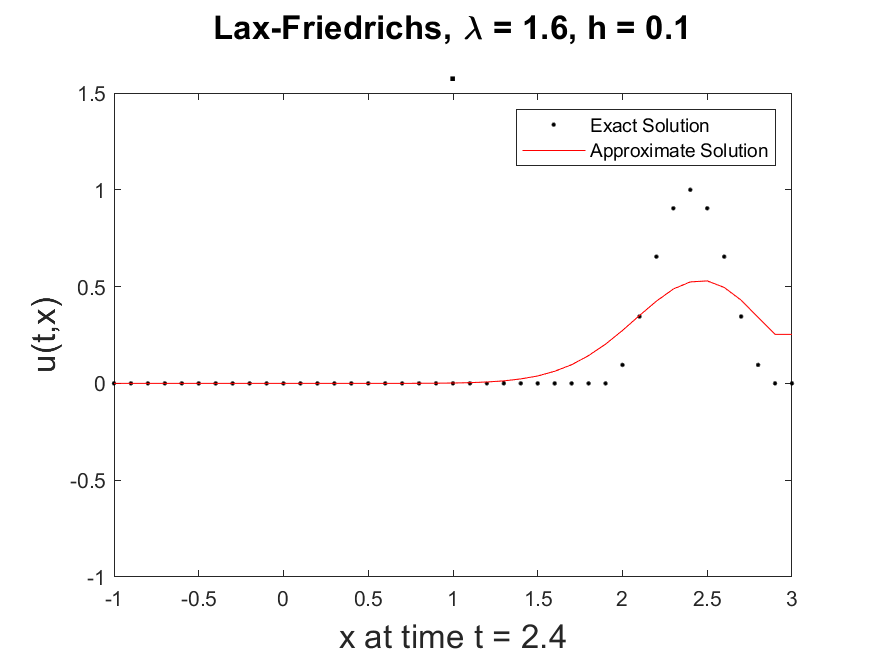
\includegraphics[width=.6\linewidth]{./code/c_lax_friedrichs_1_10th.png}	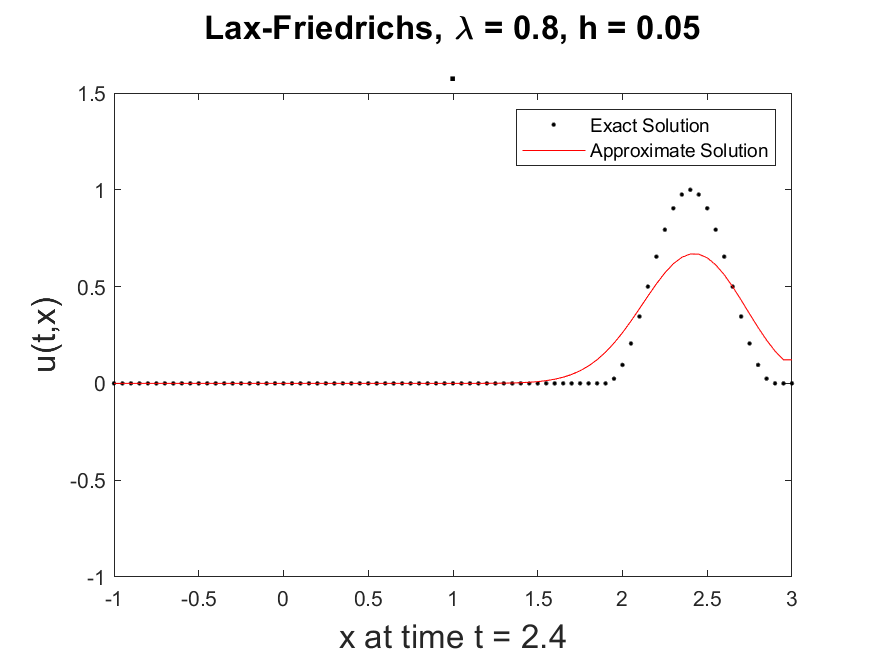
\includegraphics[width=.6\linewidth]{./code/c_lax_friedrichs_1_20th.png}
	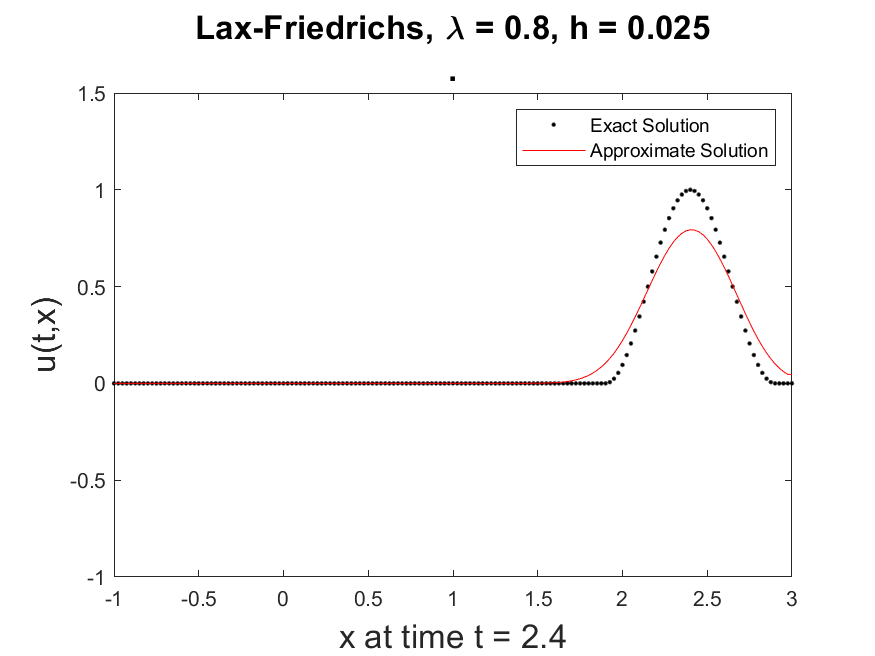
\includegraphics[width=.6\linewidth]{./code/c_lax_friedrichs_1_40th.png}
	\caption{Lax-Friedrichs at $\lambda = 0.8$ and $t=2.4$ for $h-1/10, h=1/20$, and $h=1/40$, respectively}
\end{figure}

\subsubsection*{(c$_2$) Lax-Friedrichs, $\lambda = 1.6$}
\vspace{-1mm}
Figure (4) shows this scheme. Notice that the approximate solution explodes to infinity  (see video in code). For $h=1/10$, the solution exceeds a value of 5 after about 1.44 seconds. For $h=1/20$, the solution exceeds 5 after about 1.12 seconds. For $h=1/40$, the solution passes 5 after about 0.72 seconds. As the density of the mesh doubles, the solution becomes useless about 30\% more quickly.



\begin{figure}
	\centering
	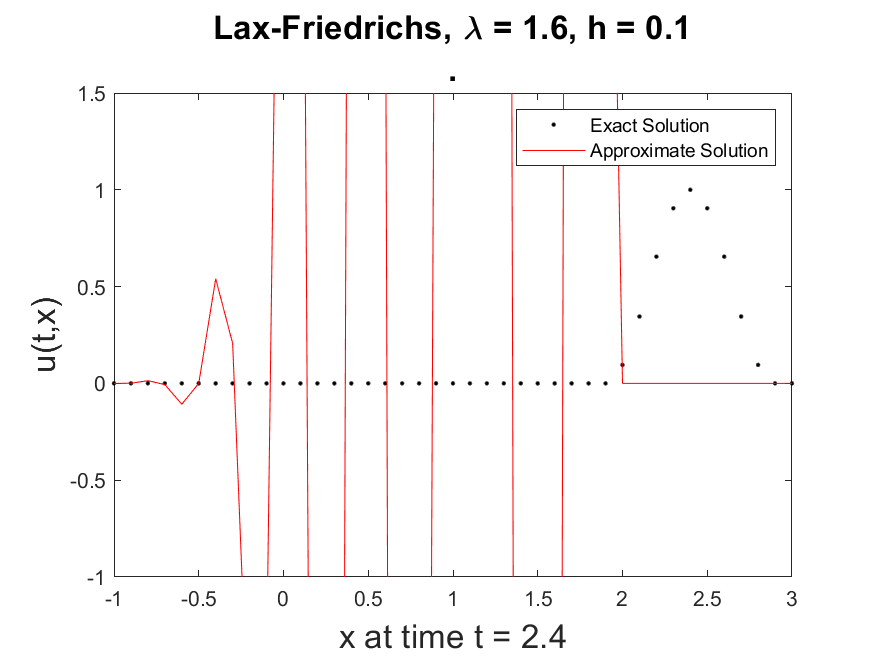
\includegraphics[width=.6\linewidth]{./code/c_lax_friedrichs_1_10th-16.png}	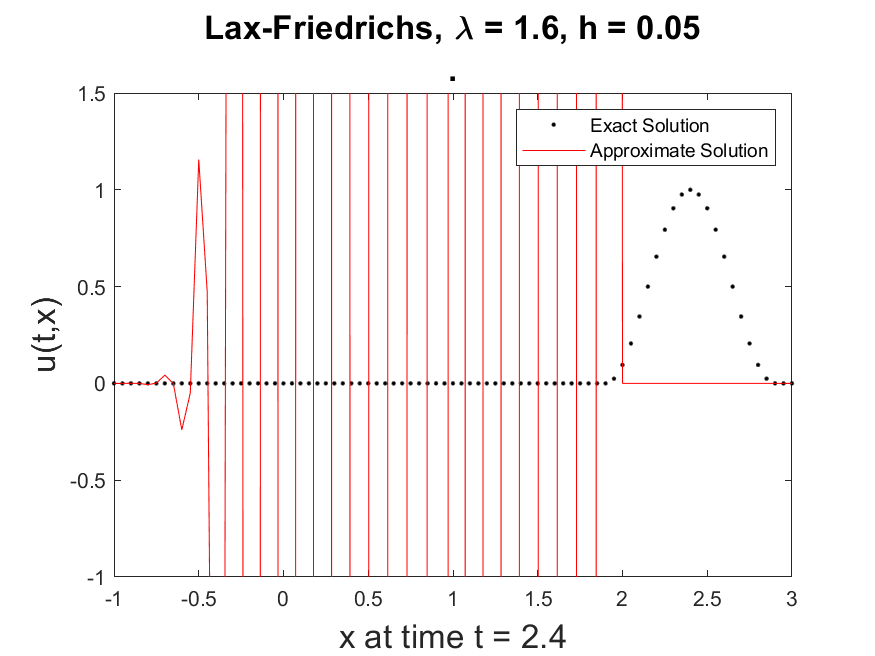
\includegraphics[width=.6\linewidth]{./code/c_lax_friedrichs_1_20th-16.png}
	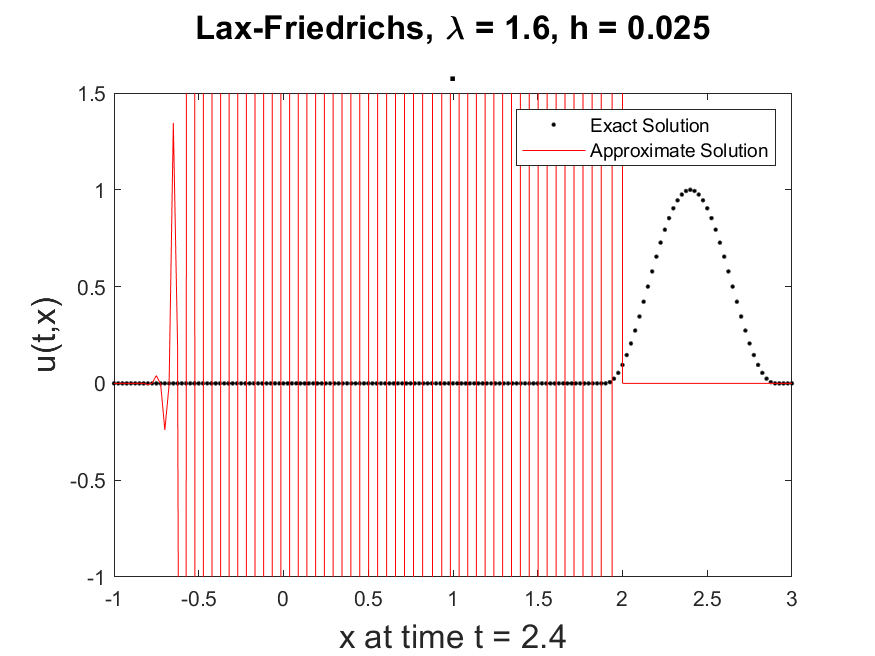
\includegraphics[width=.6\linewidth]{./code/c_lax_friedrichs_1_40th-16.png}
	\caption{Lax-Friedrichs at $\lambda = 1.6$ and $t=2.4$ for $h-1/10, h=1/20$, and $h=1/40$, respectively}
\end{figure}

\subsubsection*{(d) Leapfrog}
\vspace{-1mm}
Figure (5) shows this scheme. Notice that the approximate solution has a significant error at first, but is ultimately very useful (see video, emailed). For $h=1/10$, the error is 0.0755. For $h=1/20$, the error is 0.0151. For $h=1/40$, the error is 0.0030. As the density of the mesh doubles, the error decreases by about 3/4. This is clearly the most successful scheme.

\begin{figure}
	\centering
	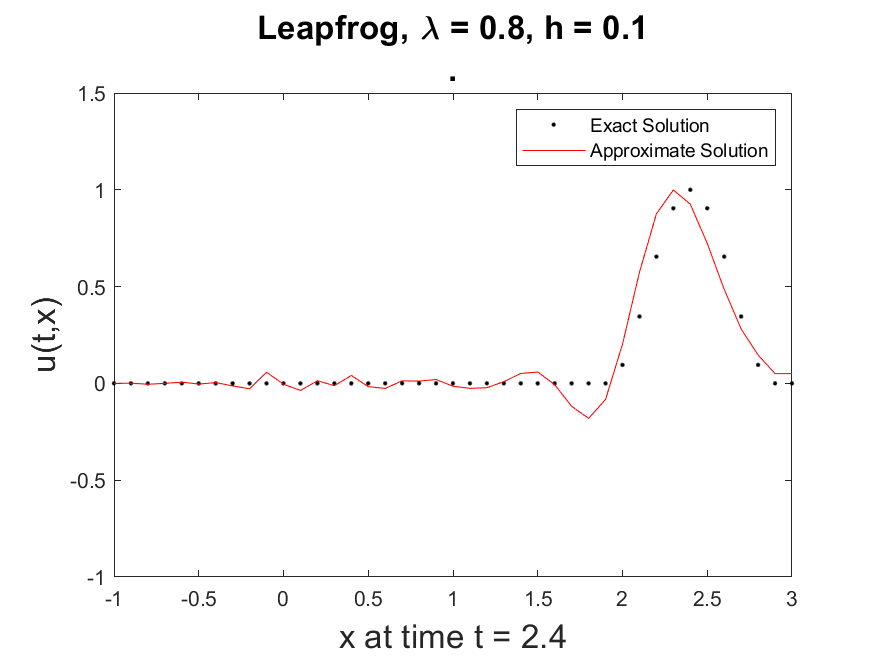
\includegraphics[width=.6\linewidth]{./code/d_leapfrog_1_10th.png}	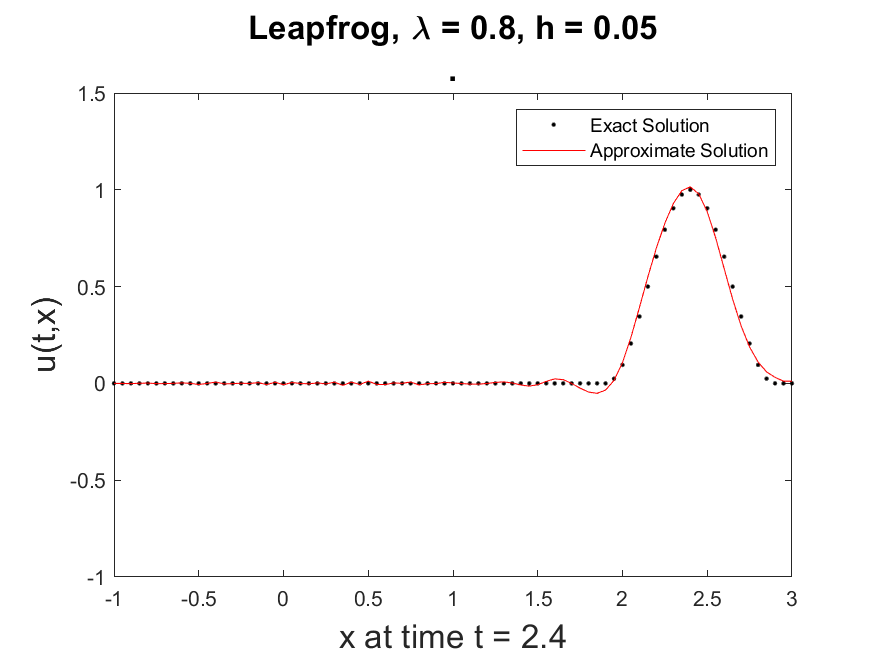
\includegraphics[width=.6\linewidth]{./code/d_leapfrog_1_20th.png}
	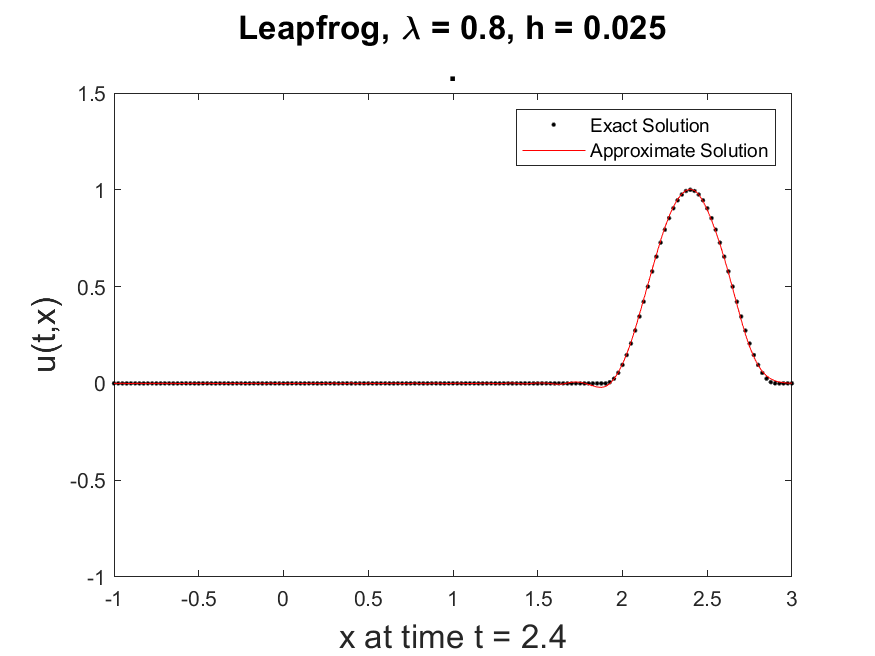
\includegraphics[width=.6\linewidth]{./code/d_leapfrog_1_40th.png}
	\caption{Leapfrog scheme at $t=2.4$ for $h-1/10, h=1/20$, and $h=1/40$, respectively}
\end{figure}

\pagebreak

\section*{1.4.2}

Show that the leapfrog scheme is consistent with the one-way wave equation.

\subsubsection*{Solution}

First, let's establish the equations we are working with. 

\begin{equation*}
\begin{aligned}
 \text{one-way wave eq.}~~~~ & P(u) = u_t + u_x = 0 \\
 \text{leapfrog scheme} ~~~~~~& P_{k,h}(u)\frac{u_m^{n+1} - u_m^{n-1}}{2k} + a\frac{u_{m+1}^n - u^n_{m-1}}{2h}
\end{aligned}
\end{equation*}

Now we write out the Taylor expansion for each term of the leapfrog scheme. The respective MATLAB commands used to quickly find the Taylor expansions for $u_m^{n+1}, ~u_m^{n-1}, ~u_{m+1}^n, ~u_{m-1}^n$ were:

\begin{verbatim}
	taylor(f(t+k, x), [h,k], 'ExpansionPoint', [0,0], 'Order', 3)
	taylor(f(t-k, x), [h,k], 'ExpansionPoint', [0,0], 'Order', 3)
	taylor(f(t, x+h), [h,k], 'ExpansionPoint', [0,0], 'Order', 3)
	taylor(f(t, x-h), [h,k], 'ExpansionPoint', [0,0], 'Order', 3)
\end{verbatim}

The Taylor expansion for these terms gives us:

\begin{equation*}
\begin{aligned}
	u_m^{n+1} = u_m^n + ku_t + \frac{1}{2}k^2u_{tt} + \mathcal{O}(k^3)\\
	u_m^{n-1} = u_m^n - ku_t + \frac{1}{2}k^2u_{tt} + \mathcal{O}(k^3)\\
	u_{m+1}^n = u_m^n + hu_x + \frac{1}{2}h^2u_{xx} + \mathcal{O}(h^3)\\
	u_{m-1}^n = u_m^n - hu_x + \frac{1}{2}h^2u_{xx} + \mathcal{O}(h^3)
\end{aligned}
\end{equation*}

Now we substitute the expansion into the leapfrog scheme, yielding:

\begin{equation*}
\begin{aligned}
	&\frac{(u_m^n + ku_t + \frac{1}{2}k^2u_{tt} + \mathcal{O}(k^3))-(u_m^n - ku_t + \frac{1}{2}k^2u_{tt} + \mathcal{O}(k^3))}{2k} - \\
	&a\frac{(u_m^n + hu_x + \frac{1}{2}h^2u_{xx} + \mathcal{O}(h^3))-( u_m^n - hu_x + \frac{1}{2}h^2u_{xx} + \mathcal{O}(h^3))}{2h}\\
	&=u_t+au_x
\end{aligned}
\end{equation*}

Next, it is necessary to subtract the expanded scheme from the original wave equation, and since they are identical, we get zero:

$$ P(u) - P_{k,h}(u) = (u_t + au_x) - (u_t + au_x) = 0 $$

Therefore, the leapfrog scheme is consistent with the one-way wave equation.

\section*{1.5.1}

Show that schemes of the form
$$
u_{m}^{n+1}=\alpha u_{m+1}^{n}+\beta u_{m-1}^{n}
$$
are stable if $|\alpha|+|\beta|$ is less than or equal to 1. Conclude that the Lax-Friedrichs scheme is stable if $|a \lambda|$ is less than or equal to 1 .


\subsubsection*{Solution}

By definition, a first order equation scheme is stable if there is an integer J such that for any positive time $T$, there is a constant $C_T$ such that

$$
\begin{array}{l}
{\qquad h \sum_{m=-\infty}^{\infty}\left|u_{m}^{n}\right|^{2} \leq C_{T} h \sum_{j=0}^{J} \sum_{m=-\infty}^{\infty}\left|u_{m}^{j}\right|^{2}} \\
~\\
{\text { ~~~~~for } 0 \leq n k \leq T, \text { with }(k, h) \in \Lambda}
\end{array}
$$

For a scheme of the form $u_{m}^{n+1}=\alpha u_{m+1}^{n}+\beta u_{m-1}^{n}$, we have:

$$
\begin{aligned}
\sum_{m=-\infty}^{\infty}\left|u_{i_{m}}^{n+1}\right|^{2} &=\sum_{m=-\infty}^{\infty}\left|\alpha u_{n}^{n}+\beta u_{m+1}^{n}\right|^{2} \\
& \leq \sum_{m=-\infty}^{\infty}|\alpha|^{2}\left|u_{m}^{n}\right|^{2}+2|\alpha|\left|\beta\left\|u_{m}^{n}\right\| u_{m+1}^{n}\right|+|\beta|^{2}\left|u_{m+1}^{n}\right|^{2} \\
& \leq \sum_{m=-\infty}^{\infty}|\alpha|^{2}\left|u_{m}^{n}\right|^{2}+|\alpha||\beta|\left(\left|u_{m}^{n}\right|^{2}+\left|u_{m+1}^{n}\right|^{2}\right)+|\beta|^{2}\left|u_{m+1}^{n}\right|^{2}\\
&=\sum_{m=-\infty}^{\infty}|\alpha|^{2}\left|u_{m}^{n}\right|^{2}+\left|\alpha\|\beta\| u_{m}^{n}\right|^{2}+\sum_{m=-\infty}^{\infty}|\alpha||\beta|\left|u_{m+1}^{n}\right|^{2}+|\beta|^{2}\left|u_{m+1}^{n}\right|^{2}
\end{aligned}$$

$$\begin{aligned}
&=\sum_{m=-\infty}^{\infty}|\alpha|^{2}\left|u_{m}^{n}\right|^{2}+|\alpha|\left|\beta \| u_{m}^{n}\right|^{2}+\sum_{m=-\infty}^{\infty}|\alpha||\beta|\left|u_{m}^{n}\right|^{2}+|\beta|^{2}\left|u_{m}^{n}\right|^{2}\\
&=\sum_{m=-\infty}^{\infty}\left(|\alpha|^{2}+2|\alpha||\beta|+|\beta|^{2}\right)\left|u_{m}^{n}\right|^{2}\\
&=(|\alpha|+|\beta|)^{2} \sum_{m=-\infty}^{\infty}\left|u_{m}^{n}\right|^{2}\\
\end{aligned}
$$

$$
\longrightarrow ~~~\sum_{m=-\infty}^{\infty}\left|v_{m}^{n+1}\right|^{2} \leq(|\alpha|+|\beta|)^{2} \sum_{m=-\infty}^{\infty}\left|v_{m}^{n}\right|^{2}
$$

$$
\longrightarrow ~~~ \sum_{m=-\infty}^{\infty}\left|v_{m}^{n}\right|^{2} \leq(|\alpha|+|\beta|)^{2 n} \sum_{m=-\infty}^{\infty}\left|v_{m}^{0}\right|^{2}
$$

This derivation also appears in Strikwerda pages 30-31. We can see that this can always be true for any n, so long as the term $(|\alpha|+|\beta|)^{2 n}$ does not approach infinity. This would be possible only if $|\alpha|+|\beta|\leq 1$.

The Lax-Friedrichs scheme is similar to this form, and the stability derivation is performed in nearly the same way:

$$
\frac{u_{m}^{n+1}-\frac{1}{2}\left(u_{m+1}^{n}+u_{m-1}^{n}\right)}{k}+a \frac{u_{m+1}^{n}-u_{m-1}^{n}}{2 h} 
$$

$$ \longrightarrow~~u_m^{n+1} = (1/2-a/2\lambda)u_{m+1}^n + (1/2+a/2\lambda)u_{m-1}^n $$

Following the previous form, we have $\alpha = 1/2-a/2\lambda$ and $\beta =1/2+a/2\lambda$. Therefore,
$$ \begin{aligned}
	|\alpha| + |\beta| & = |1/2-a/2\lambda| + |1/2+a/2\lambda|=\frac{1}{2}(|1-a\lambda| + |1+a\lambda|)\leq 1 ~~~\longrightarrow
\end{aligned} $$

$$ 2|1-a\lambda| \leq |1-a\lambda| + |1+a\lambda| \leq 2 ~~~\longrightarrow |1-a\lambda|\leq 1$$

For this equivalence to be true, we need $|a\lambda|\leq1$, which is our required term for stability.


\end{document}









